\documentclass{article}


\usepackage{arxiv}


\usepackage[utf8]{inputenc} % allow utf-8 input
\usepackage[T1]{fontenc}    % use 8-bit T1 fonts
\usepackage[hidelinks]{hyperref}       % hyperlinks
\usepackage{url}            % simple URL typesetting
\usepackage{booktabs}       % professional-quality tables
\usepackage{amsfonts}       % blackboard math symbols
\usepackage{nicefrac}       % compact symbols for 1/2, etc.
\usepackage{microtype}      % microtypography
\usepackage{lipsum}
\usepackage{tikz}
\usepackage{dsfont}
\usepackage{amsmath}
\usepackage{array}
\usepackage{todonotes}
\usepackage{float}
\usepackage{rotating}
\usepackage[toc,page]{appendix} %appendix
%\usepackage[sort&compress,square,comma,authoryear]{natbib}

\definecolor{maroon}{RGB}{176, 48, 96}
\definecolor{orange2}{RGB}{238, 118, 0}
\newcommand{\colindic}[1]{\textcolor{maroon}{#1}}
\newcommand{\colsurvey}[1]{\textcolor{orange2}{#1}}




\title{Adjusted age-specific case fatality ratio during the COVID-19 epidemic in Hubei, China, January and February 2020}

\author{
   Julien Riou \\
  Institute of Social and Preventive Medicine\\
  University of Bern\\
  Bern, Switzerland \\
  \texttt{julien.riou@ispm.unibe.ch} \\
  \And
   Anthony Hauser \\
  Institute of Social and Preventive Medicine\\
  University of Bern\\
  Bern, Switzerland \\
  \texttt{anthony.hauser@ispm.unibe.ch} \\
  \And
   Michel J.~Counotte \\
  Institute of Social and Preventive Medicine\\
  University of Bern\\
  Bern, Switzerland \\
  \texttt{michel.counotte@ispm.unibe.ch} \\
  \And
Christian L.~Althaus \\
Institute of Social and Preventive Medicine\\
University of Bern\\
Bern, Switzerland \\
\texttt{christian.althaus@alumni.ethz.ch}
}



\begin{document}

\maketitle

\begin{abstract}
The coronavirus disease 2019 (COVID-19) epidemic that originated in Wuhan, China has spread to more than 60 countries. We estimated the age-specific case fatality ratio (CFR) by fitting a transmission model to data from China, accounting for underreporting of cases and the time delay to death. Overall CFR among all infections was 1.6\% (1.4-1.8\%) and increased considerably for the elderly, highlighting the expected burden for populations with further expansion of the COVID-19 epidemic around the globe.
\end{abstract}

\section*{Introduction}

As of 2 March 2020, the 2019 novel coronavirus disease (COVID-19) epidemic that originated in Wuhan, China, has affected more than 60 countries and resulted in 88,948 confirmed cases and 3,043 deaths globally [1]. The transmission characteristics of COVID-19 appear to be similar to those of pandemic influenza and will likely facilitate further global spread [2]. During this early phase of a potential pandemic, it is critically important to obtain reliable estimates of the overall case fatality ratio (CFR), i.e., the proportion of all (asymptomatic and symptomatic) infected cases that will die as a result of the disease. Such estimates will help anticipate the expected morbidity and mortality due to COVID-19 and provide critical information for the planning of health care systems in countries that face an epidemic.

Obtaining reliable estimates of CFR can be challenging during the early phase of an epidemic [3, 4]. A crude CFR of 2.3\% was estimated based on 1,023 deaths out of 44,672 confirmed cases reported until February 11, 2020 [5]. So-called “crude estimates” of CFR from the reported numbers of confirmed cases and deaths are difficult to interpret due to the likely under-ascertainment of mild or asymptomatic cases and the right-censoring of cases with respect to the time delay from illness onset to death. Some analyses attempted to correct for right-censoring of deaths, leading to an estimate of CFR of 7.2\% (95\% confidence interval: 6.6\%-8.0\%) for Hubei province using a competing risk model [6]. Using data on exported cases and correcting for right-censoring of deaths occurred in China, another team reported a CFR estimate of 5.3\% (95\% confidence interval: 3.5\%, 7.5\%) among confirmed cases [7]. Finally, another team reported a CFR of 18\% (95\% credible interval: 11-81\%) among cases detected in Hubei, accounting for the delay in mortality [8]. The same study provided adjusted estimates of the overall CFR based on data from the early epidemic in Hubei and from cases reported outside China at 1\% (95\% CI: 0.5\%-4\%). With the objective of correcting all listed biases, we fitted a dynamic transmission model to reported data of confirmed cases and deaths in Hubei [9] and obtained adjusted and age-specific estimates of the overall CFR of COVID-19 among both symptomatic and asymptomatic patients in the Hubei province until 11 February 2020. 

\section*{The COVID-19 epidemic in Hubei, China}

The outbreak of COVID-19 appears to originate from multiple zoonotic transmission events at the Huanan Wholesale Seafood market in Wuhan in early December 2019, with the animal source remaining unknown [10]. Early January 2020, a novel coronavirus (subsequently named SARS-CoV-2) was identified as the causal agent of the epidemic [11]. In a first phase of the epidemic, human-to-human transmission occurred at a high rate in Wuhan and other areas of the Hubei province, leading to an exponential growth of incidence (Figure \ref{fig:desc}A). On 20 January, Chinese authorities implemented strict control measures in the Hubei province, including contact tracing aimed at identifying , treating and isolating cases and quarantining contacts, extension of holidays, temperature checks before accessing public areas, cancellation of mass gatherings and  the promotion of extreme social distancing [10]. Three days later, a cordon sanitaire was imposed, with strict traffic restrictions. From 27 January, the daily incidence of cases by disease onset started plateauing, then decreased. The Chinese CDC published a description of the epidemiological characteristics of cases reported until 11 February 2020, including the age distribution of cases and deaths reported up to this point in China, that we applied to Hubei (Figure \ref{fig:desc}B). 

\begin{figure}[t]
	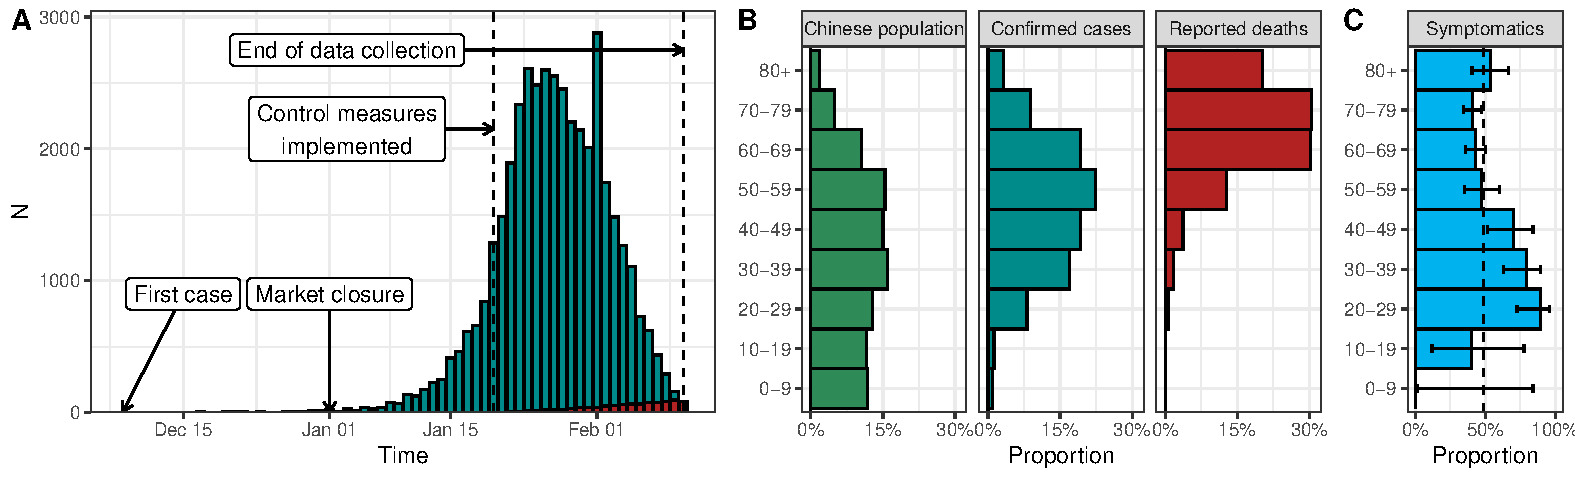
\includegraphics[width=\linewidth]{../figures/fig_desc.pdf}
	\caption{(A) Reported confirmed cases of COVID-19 in Hubei by date of disease onset (blue) and reported deaths (red) from 8 December, 2019 until 11 February, 2020. (B) Age distribution of the Chinese population compared to that of confirmed cases of and deaths due to COVID-19. (C) Proportion of individuals infected by COVID-19 showing symptoms among passengers of the Diamond Princess ship (with 95\% credible interval).}
	\label{fig:desc}
\end{figure}

\section*{An age-structured model of COVID-19 transmission and mortality}

We simulated the dynamics of the COVID-19 epidemic in Hubei from 1 January 2020 to 11 February 2020. We used an age-stratified susceptible-exposed-infected-removed (SEIR) compartmental model, with a distinction between asymptomatic and symptomatic infections. We stratified the population by 10-year ranges, leading to 9 age classes (0-9 years old, ..., 80 years old and more). After an incubation period of 5.6 days [12], 49\% of infected people develop symptoms and become infectious [13] while the remaining remain asymptomatic and do not transmit the disease further. This proportion of 49\% of symptomatic was estimated by testing every passenger on the Diamond Princess ship (Figure \ref{fig:desc}C). We then fixed the time from onset to removal to 2.9 days [14]. These parameters are identical across all age classes.

\begin{figure}[H]
	\centering
	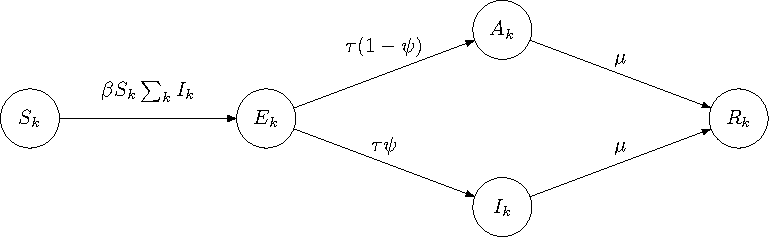
\includegraphics[width=.7\linewidth]{../figures/fig_ode.pdf}
	\caption{Schematic description of the COVID-19 transmission model. We considered five compartments for each age group $k$: susceptible $S_k$, exposed $E_k$, symptomatically infected $I_k$, asymptomatically infected $A_k$, and removed $R_k$. The cumulative incidence of symptomatic cases is recorded in compartment $C_k$, from which we compute the daily incidence of reported cases $J_k$ and the daily incidence of deaths $D_k$. Model parameters: transmission rate $\beta$, incubation rate $\tau$, probability of symptomatic infection $\psi$, removal rate $\mu$, reporting rate of symptomatics $\rho_k$ (by age group), probability of  death $\epsilon_k$ among symptomatics (by age group), and delay from disease onset to death $\gamma$ (discretized by day).}
	\label{fig:ode}
\end{figure}

We modelled the decrease in the transmission of SARS-CoV-2 due to the progressive implementation of control measures from 20 February by using a sigmoid function for the transmission rate. It includes four parameters: the initial transmission rate, the decrease in transmission due the control measures, the time delay between implementation and effect and the slope of this decrease. We assumed that symptomatic people had an age-specific case-fatality rate and that time from onset to death followed a log-normal distribution with mean 20.2 days and standard deviation 11.6 [12]. Thus, we could estimate the number of deaths at each time point and account for the deaths that occurred after 11 February 2020.

We simultaneously fitted our model to four data sets: (1) the number of confirmed cases by day of disease onset from January 1 to February 11, (2) the number of deaths by day of occurrence from January 1 to February 11, (3) the age distribution of all confirmed cases until 11 February and (4) the age distribution of all deaths reported by 11 February. These data were extracted from the CCDC report [9]. We assumed that all deaths were reported and that all symptomatic cases among people of aged 80 years and older were also reported. For the other age classes, we modelled the underreporting of symptomatic cases by an age-dependent reporting rate. We used negative binomial distributions to describe the number of reported cases and deaths and multinomial distributions to describe the distribution of cases and deaths over age classes. We implemented the model in a Bayesian framework using Stan [15]. All code and data are available from \underline{\smash{\url{https://github.com/jriou/covid_adjusted_cfr}}}.

\section*{Estimated case fatality ratio by age group during the COVID-19 epidemic in Hubei}

Our model accurately describes the dynamics of transmission and mortality by age group during the COVID-19 epidemic in Hubei from 1 January to 11 February (Figure \ref{fig:ode}). Control measures implemented on 20 January led to a reduction of transmissibility by 99\% (95\% credible interval [CrI]: 97-100), with a diminution in case incidence after six days. Under the assumption that the risk of transmission of COVID-19 was homogeneous by age, so that the deficit of reported cases in the younger age classes can be attributed to surveillance bias, the total number of symptomatic cases was estimated to 74,200 (95\%CrI: 67,000-81,600), 1.8 times more than the 41,092 reported cases during that period. Under the assumption that 49\% of infections lead to symptoms, this implies that a total of 152,700 individuals (95\%CrI: 137,800-167,900) were infected in the Hubei province during that period.

\begin{figure}[t]
	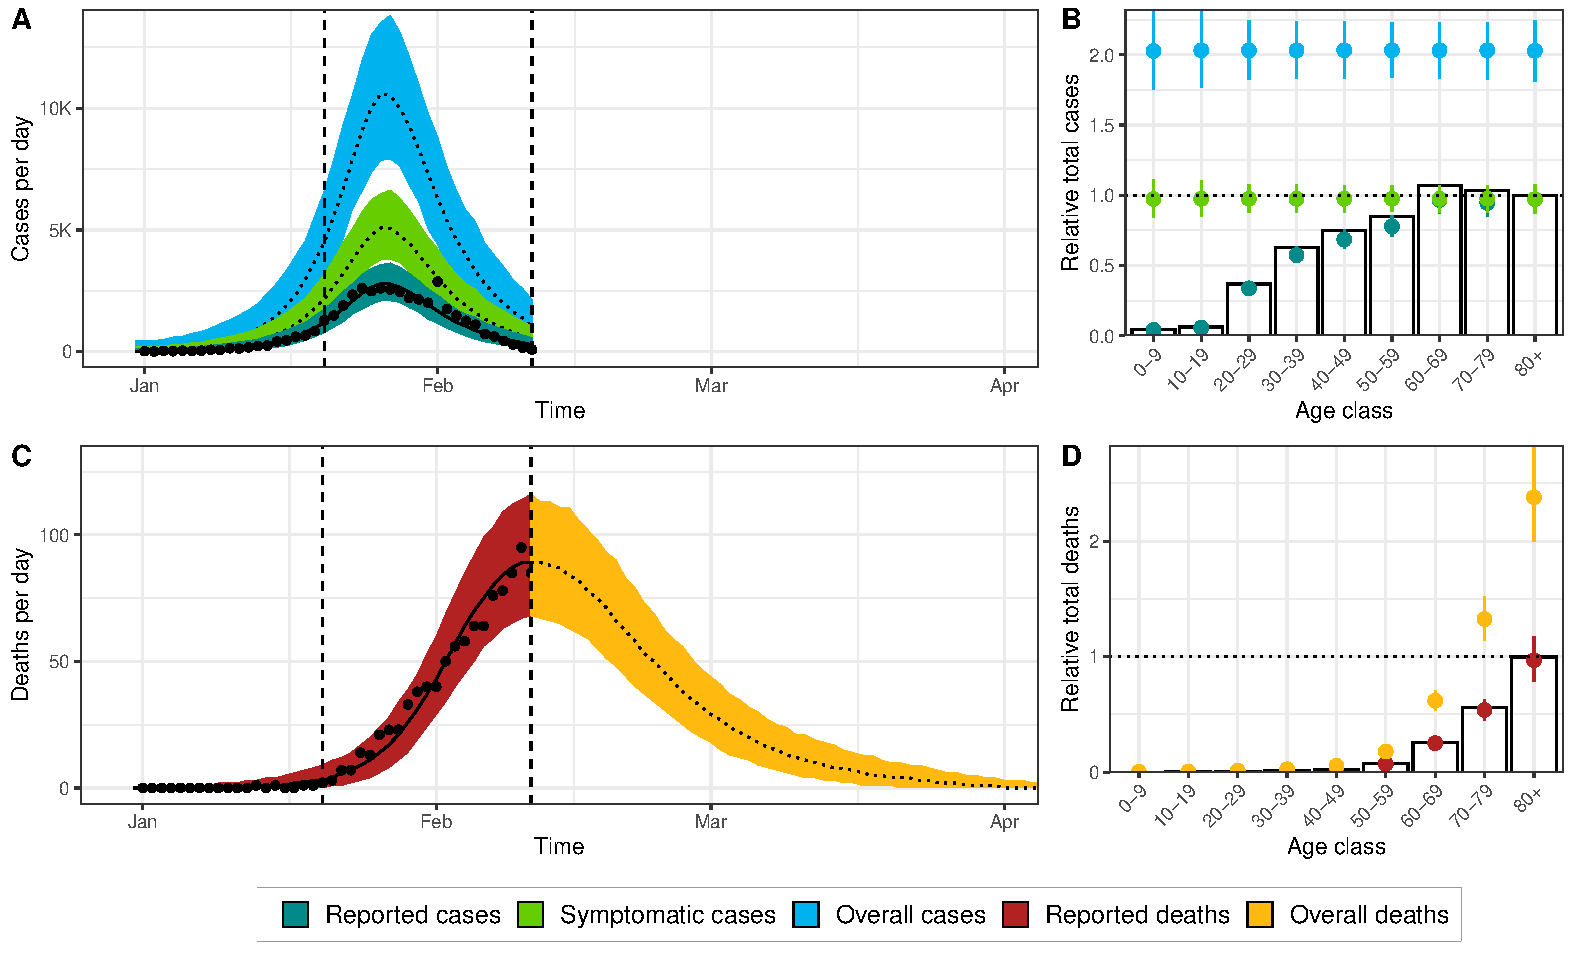
\includegraphics[width=\linewidth]{../figures/fig_fit.pdf}
	\caption{Model fit of COVID-19 incident cases (A), age distribution of cases (B), incidence of deaths (C), and age distribution of deaths (D).  Dots and columns show data. Lines and shaded areas or points and intervals show the posterior median and 95\% credible intervals for five types of model output: reported cases, symptomatic cases, overall cases (i.e. symptomatic and asymptomatic cases), reported deaths until 11 February 2020 (time point b), and deaths that will occur after this date. On panels B and D, numbers are scaled by Chinese age distribution and by the number reported for the highest age group (80+).}
	\label{fig:fit}
\end{figure}

As of 11 February, 979 deaths have been reported among people infected before that date. Under our assumption regarding the distribution of the delay between disease onset and death, the model predicts a total of 2,441 deaths (95\%CrI: 2,225-2702) among all people infected before 11 February. This results in an adjusted CFR of 1.6\% (95\%CrI: 1.4-1.8) among all people infected by COVID-19 in Hubei during that period. Moreover, our adjustment leads to sensible modifications of the age-specific CFR (Table 1). Compared to the crude CFR, the adjusted CFR is even lower in the younger age classes (0-59 years old) but higher in people aged 60 and more. 


\begin{sidewaystable}
	\caption{Estimates of case fatality ratio during the COVID-19 epidemic in Hubei, overall and by age group (median posterior and 95\% credible interval).}
	\vspace{.5em}
	
	\begin{tabular}{p{3.5cm}p{1.8cm}p{1.8cm}p{1.8cm}p{1.8cm}p{1.8cm}p{1.6cm}p{1.5cm}p{1.5cm}p{1.5cm}p{1.5cm}}
		
		\hline\\[-.8em]
		& Overall         & 0-9                & 10-19             & 20-29                & 30-39               & 40-49              & 50-59            & 60-69           & 70-79           & 80+          \\[.1em]
		\hline \\[-.8em]
		\multicolumn{10}{l}{\textit{Case fatality ratio among symptomatic infections}} \\[.4em]
		Crude & 2.4\%\hspace{4em} (2.1-2.8) & 0\%\hspace{4em} (0-1.3)        & 0.25\%\hspace{4em} (0-1.3)    & 0.22\%\hspace{4em} (0.054-0.51)  & 0.26\%\hspace{4em} (0.12-0.45)  & 0.48\%\hspace{4em} (0.28-0.73) & 1.4\%\hspace{4em} (1-1.8)    & 3.8\%\hspace{4em} (3.1-4.7) & 8.5\%\hspace{4em} (6.9-10)  & 15\%\hspace{4em} (12-18) \\[.4em]
		
		Adjusted for delayed mortality & 6\%\hspace{4em} (5.3-6.9)   & 0.44\%\hspace{4em} (0-2.8)     & 0.78\%\hspace{4em} (0-2.9)    & 0.54\%\hspace{4em} (0.18-1.2)    & 0.64\%\hspace{4em} (0.34-1.1)   & 1.2\%\hspace{4em} (0.77-1.7)   & 3.4\%\hspace{4em} (2.7-4.2)  & 9.4\%\hspace{4em} (7.9-11)  & 21\%\hspace{4em} (17-25)    & 36\%\hspace{4em} (30-44) \\[.4em]
		
		Adjusted for unidentified symptomatic cases & 1.3\%\hspace{4em} (1.2-1.5) & 0\%\hspace{4em} (0-0.055)      & 0.014\%\hspace{4em} (0-0.076) & 0.076\%\hspace{4em} (0.019-0.17) & 0.15\%\hspace{4em} (0.069-0.26) & 0.34\%\hspace{4em} (0.19-0.51) & 1.1\%\hspace{4em} (0.84-1.4) & 3.8\%\hspace{4em} (3.1-4.6) & 8.2\%\hspace{4em} (6.7-9.8) & 15\%\hspace{4em} (12-18) \\[.4em]
		
		Adjusted for both & 3.3\%\hspace{4em} (2.9-3.8) & 0.019\%\hspace{4em} (0-0.12)   & 0.046\%\hspace{4em} (0-0.17)  & 0.19\%\hspace{4em} (0.061-0.41)  & 0.38\%\hspace{4em} (0.2-0.62)   & 0.82\%\hspace{4em} (0.54-1.2)  & 2.7\%\hspace{4em} (2.1-3.4)  & 9.4\%\hspace{4em} (7.9-11)  & 20\%\hspace{4em} (17-24)    & 36\%\hspace{4em} (30-44) \\[.4em]
		\hline \\[-.8em]
		\multicolumn{10}{l}{\textit{Case fatality ratio among all symptomatic and asymptomatic infections}} \\[.4em]
		Adjusted for both & 1.6\%\hspace{4em} (1.4-1.8) & 0.0094\%\hspace{4em} (0-0.058) & 0.022\%\hspace{4em} (0-0.082) & 0.091\%\hspace{4em} (0.03-0.2)   & 0.18\%\hspace{4em} (0.096-0.3)  & 0.4\%\hspace{4em} (0.26-0.58)  & 1.3\%\hspace{4em} (1-1.6)    & 4.6\%\hspace{4em} (3.8-5.4) & 9.8\%\hspace{4em} (8.2-12)  & 18\%\hspace{4em} (14-22) \\[.4em]
		\hline
	\end{tabular}
	
	
	
\end{sidewaystable}



\section*{Strengths and limitations}

In this work, we propose a comprehensive solution to the estimation of CFR from surveillance data during outbreaks [3], and apply it to data from the COVID-19 epidemic in Hubei, China. Our work has three important strengths. (1) We use a mechanistic model for the transmission of and the mortality associated with COVID-19 that is a direct translation of the data-generating mechanisms leading to the biased observations of the number of deaths (because of right-censoring) and of cases (because of surveillance bias). Our model also accounts for the effect of control measures on disease transmission. (2) Our model is stratified by age group, which has been shown as a crucial feature for modelling emerging respiratory infections [16]. (3) The estimates rely on routinely collected surveillance data such as incident cases by disease onset, incidence deaths, and the age distribution of cases and deaths, and does not require individual-level data nor studies in the general population. The Bayesian framework allows the propagation of the uncertainty from data to the estimates.

Our work has several limitations. (1) Our results depend on the central assumption that the cause of the deficit of reported cases among younger age groups is a surveillance bias and does not reflect a lower risk of infection in younger individuals. The reason for this age shift is unknown [10]. Retrospective testing for COVID-19 of samples from influenza-like-illness surveillance found no positive test among children, but the sample sizes were small (20 per week including both adults and children) [10]. Uneven age distributions in the risk of infection can be attributed to immunological features, such as the lower circulation of H1N1 influenza in older individuals due to residual immunity [17]. An immunological explanation of the opposite phenomenon, with a lower susceptibility of younger individuals, seems unlikely, and there is no indication of pre-existing immunity to COVID-19 in humans [10]. Different contact patterns could play a role in a limited outbreak, but not in such a widespread infection, especially as household transmission seems to play a major role [10]. The last explanation that we assume here is that younger individuals, when symptomatic, have milder symptoms that decrease the probability of seeking care and being identified. 

(2) In a related matter, our results depend on the assumption that older individuals have more severe symptoms and are more likely to be identified. In the absence of an outside reference point, the reporting rate cannot be estimated from surveillance data only. We chose to fix to 100\% the reporting rate of infected individuals that have symptoms and are aged 80 and more, and estimate the reporting rates in other age groups relatively to that of older individuals. If further data, coming from a study in the general population, shows that this assumption is violated, this would lead to an overestimation of the CFR in our study.

(3) There is important uncertainty around the proportion of asymptomatic infections. Currently, the detection of asymptomatic patients in China is limited by the focus on symptomatic patients seeking care and the lack of seroprevalence data [18]. The proportion of symptomatic infections has been estimated to 58\% (95\% confidence interval: 33-83) in a small sample of cases exported to Japan [19]. During the outbreak on the ship “Diamond Princess”, nearly all individuals were tested regardless of symptoms, leading to an average proportion of symptomatic infections of 49\% in a sample size of 619, which was used in the present study [13]. Still, uncertainty about the proportion of symptomatic infections will remain until a large retrospective seroprevalence study is conducted in the general population, and our results are dependent on this estimate. Additionally, the dichotomization of infection into asymptomatic and symptomatic is a simplification of reality; the infection with SARS-CoV-2, will likely cause a gradient of symptoms in different individuals depending on age, sex and comorbidities [10]. The proportion of asymptomatic infections might show an age-dependent structure.

(4) Our findings regarding the CFR are specific to the context, and should be interpreted in that light. The findings describe the situation in Hubei from 1 January to 11 February, 2020. It was demonstrated there, that mortality rates have changed over time as a result of an improvement of the standard of care [10]. The standard of care and, as a result, the CFR is setting-dependent and cannot be directly applied to other contexts.

\section*{Conclusions}

We developed a mechanistic approach to correct for the biases in the crude estimates of CFR and provide an adjusted CFR by age group with regards to the ongoing COVID-19 epidemic in Hubei, China between 1 January and 11 February. We find that 1.6\% (1.4-1.8) of individuals infected with COVID-19 during that period with or without symptoms died or will die, with even more important differences by age group than suggested by the raw data. The probability of death among infected individuals with symptoms is estimated at 3.3\% (2.9-3.8), with a steep increase over 60 years old to reach 36\% over 80 years old. While specific to the situation in Hubei, China during this period, these findings will help the mitigation efforts and planning of resources as other regions prepare for COVID-19 epidemics. 




\section*{References}

\begin{enumerate}
	 

\item World Health Organization. Coronavirus disease 2019 (COVID-19) Situation Report 41. 2020  02/03/2020]; Available from: https://www.who.int/docs/default-source/coronaviruse/situation-reports/20200301-sitrep-41-covid-19.pdf?sfvrsn=6768306d\_2.
\item	Riou, J. and C.L. Althaus, Pattern of early human-to-human transmission of Wuhan 2019 novel coronavirus (2019-nCoV), December 2019 to January 2020. Eurosurveillance, 2020. 25(4).
\item	Lipsitch, M., et al., Potential biases in estimating absolute and relative case-fatality risks during outbreaks. PLoS neglected tropical diseases, 2015. 9(7).
\item	Battegay, M., et al., 2019-novel Coronavirus (2019-nCoV): estimating the case fatality rate–a word of caution. Swiss Medical Weekly, 2020. 150(0506).
\item	The Novel Coronavirus Pneumonia Emergency Response Epidemiology, T., The Epidemiological Characteristics of an Outbreak of 2019 Novel Coronavirus Diseases (COVID-19) — China, 2020. China CDC Weekly, 2020. 2(8): p. 113-122.
\item	Wang, X., et al., Estimating the case fatality ratio of the COVID-19 epidemic in China. medRxiv, 2020.
\item	Jung, S.-m., et al., Real-Time Estimation of the Risk of Death from Novel Coronavirus (COVID-19) Infection: Inference Using Exported Cases. Journal of Clinical Medicine, 2020. 9(2): p. 523.
\item	Dorigatti, I., et al. Report 4: Severity of 2019-novel coronavirus (nCoV) 2020  03/03/2020]; Available from: https://www.imperial.ac.uk/media/imperial-college/medicine/sph/ide/gida-fellowships/Imperial-College-2019-nCoV-severity-10-02-2020.pdf.
\item	Team, T.N.C.P.E.R.E., Vital Surveillances: The Epidemiological Characteristics of an Outbreak of 2019 Novel Coronavirus Diseases (COVID-19) — China, 2020. China CDC Weekly, 2020. 2(8): p. 113-122.
\item	World Health Organization-China Joint Mission on Coronavirus Disease 2019 Group. Report of the WHO-China Joint Mission on Coronavirus Disease 2019 (COVID-19). 2020  02/03/2020]; Available from: https://www.who.int/docs/default-source/coronaviruse/who-china-joint-mission-on-covid-19-final-report.pdf.
\item	Zhou, P., et al., A pneumonia outbreak associated with a new coronavirus of probable bat origin. Nature, 2020: p. 1-4.
\item	Linton, N.M., et al., Incubation Period and Other Epidemiological Characteristics of 2019 Novel Coronavirus Infections with Right Truncation: A Statistical Analysis of Publicly Available Case Data. Journal of Clinical Medicine, 2020. 9(2): p. 538.
\item	Japanese National Institute of Infectious Diseases. Field Briefing: Diamond Princess COVID-19 Cases. 2020  02/03/2020]; Available from: https://www.niid.go.jp/niid/en/2019-ncov-e/9407-covid-dp-fe-01.html.
\item	Liu, T., et al. Transmission dynamics of 2019 novel coronavirus (2019-nCoV). 2020  2020-3-3]; Available from: https://ssrn.com/abstract=3526307 
\item	Carpenter, B., et al., Stan: A probabilistic programming language. Journal of statistical software, 2017. 76(1).
\item	Pellis, L., et al., Systematic selection between age and household structure for models aimed at emerging epidemic predictions. Nature Communications, 2020. 11(1): p. 1-11.
\item	Pérez-Trallero, E., et al., Residual immunity in older people against the influenza A (H1N1)–recent experience in northern Spain. Eurosurveillance, 2009. 14(39): p. 19344.
\item	Carrat, F., et al., Time lines of infection and disease in human influenza: a review of volunteer challenge studies. American journal of epidemiology, 2008. 167(7): p. 775-785.
\item	Nishiura, H., et al., Estimation of the asymptomatic ratio of novel coronavirus infections (COVID-19). medRxiv, 2020.
\end{enumerate}


\section*{Acknowledgements}
JR is funded by the Swiss National Science Foundation (grant 174281). MC is funded
by the Swiss National Science Foundation (grant 176233).
\section*{Conflict of interest}
None.

\section*{Authors' contributions}

JR and AH designed the model and performed the statistical analyses. JR, AH, MC
and CLA interpreted the results and wrote the manuscript.


\end{document}
